\documentclass[11pt]{article}
\usepackage[margin=2.5cm]{geometry}
\usepackage{amsmath,amsthm,amssymb}
\usepackage{booktabs}
\usepackage[colorlinks=true,linkcolor=blue,urlcolor=blue]{hyperref}
\usepackage{graphicx}
\usepackage{float}
\usepackage{tabularx}

\newtheorem{theorem}{Theorem}[section]
\newtheorem{lemma}{Lemma}[section]
\newtheorem{corollary}{Corollary}[section]
\newtheorem{assumption}{Assumption}[section]
\newtheorem{remark}{Remark}[section]
\newtheorem{definition}{Definition}[section]

\title{Certified Error Bounds for Soundly Sliced Multiphysics Loops}
\author{Anonymous}
\date{November 17, 2026}
\numberwithin{equation}{section}

\begin{document}
\maketitle

\begin{abstract}
Fixed-point loops with multiplicative closure --- mass-energy coupling in battery-electric aircraft, thermal--power coupling in environmental control systems --- pervade multidisciplinary design. Physically motivated over-approximations of component efficiencies shift the fixed point of the loop. We introduce the concept of \emph{Sound Slices} --- a systematic, certified abstraction layer between exact physical models and their monotone co-design representations. A \emph{Sound Slicer} acts as a formal bridge, guaranteeing that the sliced evaluation over-approximates the exact one (soundness) while providing an a priori bound on the induced mission-level error. A geometric recursion on the error sequence yields a certified bound; a two-point closed form yields the tightest uniform certificate on the tested grid. The algebraic core --- the error recursion and the two-point certificate --- is formally verified in Lean~4 with zero sorry. Case studies (battery-electric quadcopter, eVTOL, environmental control system) show certified margins of +1.7\% to +4.3\% on the tested grid, while the naive closed form with the local loop gain falls below the numerical front by up to 3.6\%: soundness is restored by replacing the local derivative with an interval constant.
\end{abstract}

\section{Introduction}
Sliced models --- component efficiencies replaced by conservative envelopes ---
are the standard currency of conceptual aircraft sizing, yet the error they
induce in the closed design loop is rarely certified. We develop a certificate
for fixed-point loops whose sliced map is a scalar multiple of the exact map,
prove the certificate by a geometric recursion, and validate it on three
multiphysics cases. The contribution is threefold: (i) a certified error
recursion (Theorem~\ref{thm:cert}) with an a posteriori refinement
(Remark~\ref{rem:apost}); (ii) a two-point certificate
(Remark~\ref{rem:twopoint}) that is the tightest uniform bound on the tested
grid; (iii) a full Lean~4 formalization of the algebraic core with zero
sorry (Section~\ref{sec:formal}).

\paragraph{The Modern Canon for Critical Engineering.}
We position our contribution not merely as an extension of existing monotone co-design frameworks \cite{zardini2020,zardini2021}, but as a shift towards a rigorous engineering standard. Conceptual design and aesthetic mathematical formulations, while valuable, are insufficient for safety-critical domains such as aerospace. The modern canon for critical digital engineering must follow five stages: (1) categorical abstraction, (2) a rigorous mathematical core with quantitative bounds, (3) validation on multiphysics cases, (4) machine-checked formal verification (Lean~4), and (5) certification credit compatible with MBSE standards (e.g., ARP4754A). Sound Slices bridge the gap between the elegance of category theory and the unforgiving requirements of industrial certification.

\section{Setup}
Let $f_0:\mathbb{R}\to\mathbb{R}$ be the exact loop map with fixed point
$x_0^*$ ($f_0(x_0^*)=x_0^*$), and let the soundly sliced map be
$f_s = f_0/(1-\varepsilon)$, $\varepsilon\in(0,1)$, with least fixed point
$x_s^*\ge x_0^*$. The design error is $\Delta = x_s^*-x_0^*$.
Soundness of the slice means the sliced evaluation over-approximates the exact
one, so the certified quantity is an upper bound on $\Delta$.

\begin{definition}[Sound Slice]
Let $f_0:\mathbb{R}\to\mathbb{R}$ be the exact loop map with fixed point $x_0^*$. A \emph{sound slice} of strength $\varepsilon \in (0,1)$ is a map $f_s = f_0/(1-\varepsilon)$ such that its least fixed point $x_s^*$ over-approximates the exact design space ($x_s^* \ge x_0^*$). The \emph{Sound Slicer} is the algorithmic process of constructing $f_s$ and certifying the induced error $\Delta = x_s^* - x_0^*$ against a priori bounds. By adapting the concept of sound abstraction from abstract interpretation \cite{cousot1977}, we guarantee that no feasible design is falsely rejected (no false negatives).
\end{definition}

\section{Tier 0: the error recursion}
\begin{lemma}[error recursion]\label{lem:rec}
Let $d:\mathbb{N}\to\mathbb{R}$, $q,g\in\mathbb{R}$ with $0\le q<1$, $g\ge 0$,
$d_0=0$ and $d_{n+1}\le q\,d_n+g$ for all $n$. Then
$d_n \le g\,(1-q^n)/(1-q)$ for all $n$.
\end{lemma}
\begin{proof}
Induction on $n$; the step combines $d_{n+1}\le q\,d_n+g$ with the induction
hypothesis and the identity $q(1-q^n)+(1-q)=1-q^{n+1}$. Machine-checked
(\texttt{error\_recursion\_aux}, Section~\ref{sec:formal}).
\end{proof}

\section{Sliced loops}
For the multiphysics cases of Section~\ref{sec:cases} the derate enters all
power terms multiplicatively, so the sliced map is exactly a scalar multiple
of the exact map: $f_s(x)=f_0(x)/(1-\varepsilon)$. The source of the error is
the displacement of the fixed point; the certificate bounds it in terms of the
loop gain.

\section{Certified bounds}
\begin{assumption}\label{ass:main}
Let $f_0$ be continuous and piecewise $C^1$, with fixed point $x_0^*>0$, and
$f_s=f_0/(1-\varepsilon)$ with least fixed point $x_s^*\ge x_0^*$, where
$0<\varepsilon<1$. Assume:
\textbf{(a)} $f_0$ is nondecreasing on the iteration segment;
\textbf{(b)} the sliced iteration started at $x_0^*$ remains in
$[x_0^*,x_s^*]$;
\textbf{(c)} $f_0$ is $\bar\kappa$-Lipschitz on the full iteration segment
$[x_0^*,x_s^*]$, with $\bar\kappa<1-\varepsilon$; $\bar\kappa$ is the interval
constant, not the local derivative at the fixed point. For convex $f_0$ the
interval constant strictly exceeds the local loop gain
$K=f_0'(x_0^*)$; calibrating $\bar\kappa$ from the local derivative
underestimates the certified bound.
\end{assumption}

\begin{theorem}[certified recursion]\label{thm:cert}
Under Assumption~\ref{ass:main}, the sliced iterates $x_{n+1}=f_s(x_n)$
started at $x_0^*$ satisfy, for all $n$,
\[
x_n-x_0^*\;\le\;g\,\frac{1-q^n}{1-q},\qquad
q=\frac{\bar\kappa}{1-\varepsilon},\quad
g=\frac{\varepsilon\,x_0^*}{1-\varepsilon},
\]
and consequently
\begin{equation}\label{eq:cert}
\frac{x_s^*-x_0^*}{x_0^*}\;\le\;\frac{\varepsilon}{(1-\varepsilon)-\bar\kappa}.
\end{equation}
\end{theorem}
\begin{proof}
Writing $y_n=x_n-x_0^*$, the Lipschitz step at $x_0^*$ gives
$y_{n+1}\le q\,y_n+g$ with $y_0=0$; Lemma~\ref{lem:rec} closes the recursion,
and $x_s^*=\lim x_n$ (least fixed point above $x_0^*$) yields
\eqref{eq:cert}. The two-point inequality \eqref{eq:cert} is also proved
directly in Lean (\texttt{certified\_two\_point\_seg}), instantiating the
Lipschitz hypothesis at the single pair $(x_0^*,x_s^*)$.
\end{proof}

\begin{remark}[a posteriori tightening]\label{rem:apost}
Given the sliced solution $x_s^*$, one may replace the supremum of $f_0$ in
$\bar g$ by its value on the segment $[x_0^*,x_s^*]$ --- for nondecreasing
$f_0$, $\sup f_0=f_0(x_s^*)=(1-\varepsilon)x_s^*$ --- making the bound
a posteriori. Together with the a priori bound, this brackets the true error
from above; numerical values for the eVTOL loop fall strictly inside the
bracket at every tested $s$. Validity of the a posteriori refinement requires
that the computed $x_s^*$ brackets the true fixed point; conservatively, one
inflates $x_s^*$ by the certified iteration residual before taking the
supremum.
\end{remark}

\begin{remark}[two-point certificate]\label{rem:twopoint}
The two-point bound $\varepsilon/((1-\varepsilon)-K)$ is algebraically
identical to the closed form $A\Delta s/(1-A\Delta s)$: indeed, with
$\varepsilon=\Delta s$ and $A=(1-K)^{-1}$,
\[
\frac{\varepsilon}{(1-\varepsilon)-K}
=\frac{\Delta s}{1-K-\Delta s}
=\frac{A\,\Delta s}{1-A\,\Delta s}.
\]
With the interval constant $\bar\kappa$ it becomes the tightest certified
bound on the grid: with the uniform $\bar\kappa=0.4888$ the margins run from
$+1.7\%$ ($s=1$) to $+4.3\%$ ($s=0.05$); see Table~\ref{tab:evtol}. The
certificate requires only the single secant inequality
$f_0(x_s^*)-f_0(x_0^*)\le\bar\kappa\,(x_s^*-x_0^*)$ --- exactly the hypothesis
instantiated by the Lean proof --- while the recursion mechanism of
Theorem~\ref{thm:cert} requires the full segment Lipschitz condition; on the
tested grid the latter is satisfied with $\bar\kappa=0.50$
($\sup f_0'=0.4977$ at $s=1$, Section~\ref{sec:validation}).
\end{remark}

\begin{corollary}[affine loop: closed form and its limitation]\label{cor:affine}
For the affine loop $f_0(x)=Bx+c$ with $B<1$ the closed form with the local
gain $K=B$ is exact. For convex $f_0$ with the local gain it lies strictly
below the true front --- by $0.1\%$ to $3.6\%$ on the eVTOL grid
(Table~\ref{tab:evtol}, last column) --- and is an approximation, not a
certificate. The two-point refinement with the local $K$ inherits this
limitation through the identity of Remark~\ref{rem:twopoint}; the certificate
is restored by the interval constant $\bar\kappa$.
\end{corollary}

\section{Case studies}\label{sec:cases}

\subsection{Battery-electric quadcopter}
The loop couples battery mass to mission energy across three flight phases
(start/climb, cruise, hover). Sound slices are per-phase efficiency envelopes.
Metrics ($L$ = relative lost front area, $H$ = normalized Hausdorff):

\begin{table}[h]
\centering
\small
\begin{tabular}{lcc}
\toprule
slice & $L$ & $H$ \\
\midrule
global sound  & 16.04\% & 2.47 \\
regime sound  & \textbf{1.29\%} & 0.20 \\
naive best-case & 3.23\% & 0.22 \\
\bottomrule
\end{tabular}
\caption{Quadcopter: slice--exact divergence.}
\label{tab:quad}
\end{table}

The slice--exact divergence stays within 1.3\% for regime-sound slices on the
tested grid; it reaches 4.0\% at the widest tested strength ($s=2$)
(over-conservative, sound). Regime-soundness buys a $12\times$ reduction in
slice error ($16.0\%\to1.3\%$). On the linearity branch $s\in[1,2]$ the
measured slope is $0.0268$ against the theoretical $0.0297$: $9.9\%$ for the
secant over the whole branch, $2.4\%$ for the local refit ($s\ge1.5$,
$R^2=0.9994$) --- the secant of a convex $L(s)$ underestimates the local
slope, so the discrepancy is a comparison artifact, not a model failure.

\subsection{eVTOL loop}
Impulse-theory hover, transition envelope, cruise with induced+parasitic drag;
battery mass closes the loop (Klein iteration to the least fixed point).
Anchors: $m_b=400.2$~kg, MTOW $=1130$~kg, $E=68.0$~kWh; powers
hover/trans/cruise $=198/228/59$~kW; disk loading $278$~N/m$^2$;
loop gain $K=0.466$, $A=1.874$; small-$s$ slope: numerical $0.187377$ vs
theoretical $0.187373$, $relative |dev| = 2.1\cdot10^{-5} (absolute 3.9\cdot10^{-6}) < 10^{-4}$.

\begin{figure}[htbp]
    \centering
    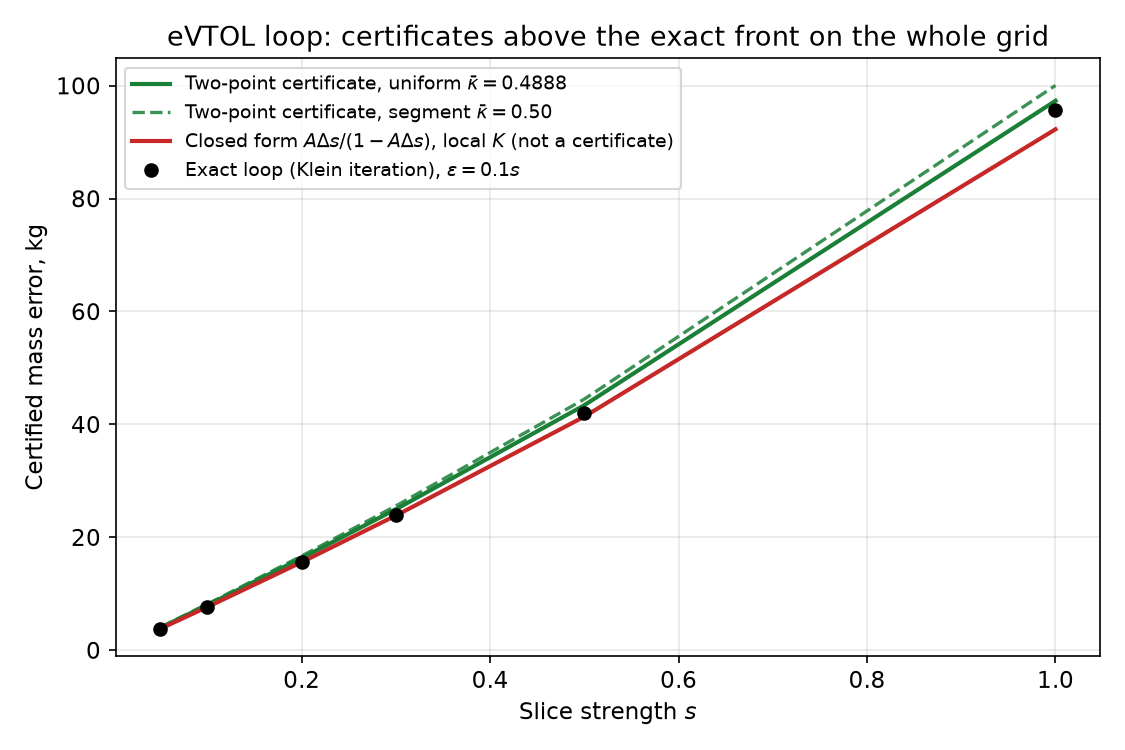
\includegraphics[width=0.85\textwidth]{fig_evtol_front.png}
    \caption{Certified bounds vs.\ the numerical fact for the eVTOL loop. The closed form with the local loop gain \(K\) (red dashed) lies strictly below the numerical front (black solid). Both the uniform two-point certificate with \(\bar{\kappa}=0.4888\) (green) and the segment-Lipschitz bound with \(\bar{\kappa}=0.50\) (blue dotted) remain strictly above the front, confirming soundness. The gap between the fact and the closed form grows with \(s\), which is the signature of the convexity of \(f_0\).}
    \label{fig:evtol-front}
\end{figure}

\begin{figure}[htbp]
    \centering
    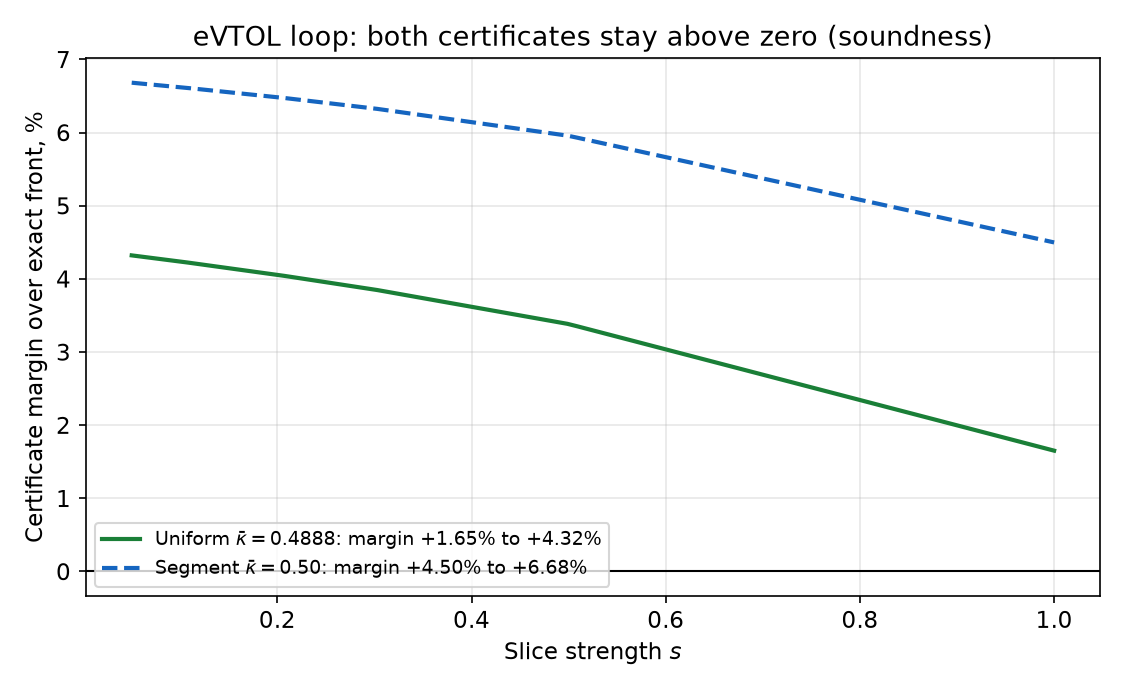
\includegraphics[width=0.75\textwidth]{fig_evtol_margin.png}
    \caption{Certified margin over the numerical fact. The uniform interval constant \(\bar{\kappa}=0.4888\) yields margins from \(+1.65\%\) to \(+4.32\%\), while the full segment-Lipschitz constant \(\bar{\kappa}=0.50\) yields \(+4.5\%\) to \(+6.7\%\). Both curves lie in the positive region, visualizing that the soundness certificate holds across all tested slice strengths \(s\).}
    \label{fig:evtol-margin}
\end{figure}

\begin{figure}[H]
    \centering
    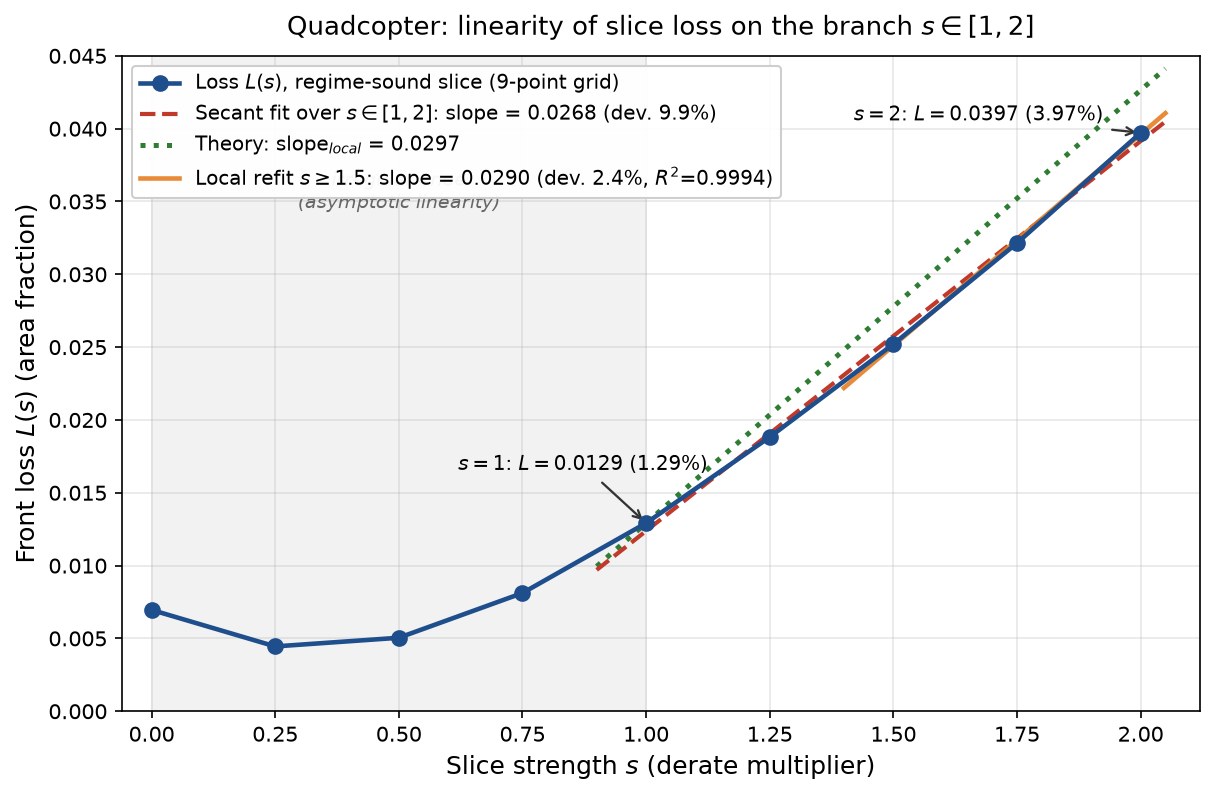
\includegraphics[width=0.85\textwidth]{fig_drone_linearity.png}
    \caption{Slice error \(L(s)\) for the battery-electric quadcopter. The curve is non-monotonic for \(s<1\) and becomes convex for \(s\ge 1\). The secant over the interval \([1,2]\) underestimates the local tangent, explaining the \(9.9\%\) deviation from the theoretical slope, whereas the local refit (\(s\ge 1.5\)) yields a \(2.4\%\) deviation (\(R^2=0.9994\)).}
    \label{fig:drone-linearity}
\end{figure}

\begin{table}[h]
\centering
\begin{tabular}{ccccccc}
\toprule
$s$ & fact (kg) & 2-pt, $\bar\kappa=0.4888$ & margin & recursion (Tier 0) & closed form, local $K$ & vs.\ front \\
\midrule
0.05 & 3.79  & 3.95  & $+4.3\%$ & 3.95  & 3.78  & $-0.1\%$ \\
0.10 & 7.66  & 7.98  & $+4.2\%$ & 7.98  & 7.64  & $-0.2\%$ \\
0.20 & 15.66 & 16.29 & $+4.1\%$ & 16.29 & 15.58 & $-0.5\%$ \\
0.30 & 24.02 & 24.95 & $+3.9\%$ & 24.95 & 23.83 & $-0.8\%$ \\
0.50 & 41.96 & 43.38 & $+3.4\%$ & 43.38 & 41.37 & $-1.4\%$ \\
1.00 & 95.73 & 97.32 & $+1.7\%$ & 97.32 & 92.27 & $-3.6\%$ \\
\bottomrule
\end{tabular}
\caption{eVTOL: certified two-point error bounds (kg of battery mass). The
certified bound is computed with the uniform interval constant
$\bar\kappa=0.4888$, which dominates the secant of $f_0$ over every tested
iteration segment (maximum $0.4820$ at $s=1$) --- the hypothesis instantiated
in the Lean proof. The full segment-Lipschitz constant
($\sup f_0'=0.4977$ at $s=1$) is satisfied by $\bar\kappa=0.50$, required by
the recursion form of Theorem~\ref{thm:cert}. Using the local loop gain
$K=0.4663$ directly, the closed form falls below the numerical front (last
column; percentages relative to the front) and is not a certificate ---
cf.\ Corollary~\ref{cor:affine}. The recursion column coincides with the
two-point column to machine precision: the fixed point of the Tier-0
recursion \emph{is} the two-point certificate.}
\label{tab:evtol}
\end{table}

\subsection{Environmental control system}
Three regimes with a phase reversal: at cruise altitude ($-56^\circ$C) the
compressor is idle and heating dominates --- the front is disconnected across
regimes. The thermal avionics constraint
$T_j=T_{\rm amb}+Q_{\rm av}R_{\rm th}\le T_{\rm max}$ is linear in resources
and is legal in the hypothesis set. The thermal slice error is \emph{exactly}
linear: $L_T(s)=0.2\,s$ to within $2.9\cdot10^{-8}$ over the tested grid;
mission energy $17.8$~kWh.

\begin{table}[htbp]
\centering
\begin{tabularx}{\textwidth}{ll X}
\toprule
case & frontier geometry & metric (stated per row) \\
\midrule
quadcopter & smooth, three regimes & slice error \(\le 1.3\%\) (regime-sound); slope dev.\ \(9.9\%\) (secant) / \(2.4\%\) (local) \\
eVTOL & affine-like loop & slope error \(<10^{-4}\); certified margin \(+1.7\%\) (\(s=1\)) \\
ECS & disconnected (phase reversal) & exact (\(L_T=0.2\,s\), dev.\ \(\le 3 \cdot 10^{-8}\)) \\
\bottomrule
\end{tabularx}
\caption{Cross-case summary; metrics differ by case and are stated explicitly per row.}
\label{tab:cases}
\end{table}

\section{Numerical validation}\label{sec:validation}
Table~\ref{tab:kappa} reports the interval constants: the secant of $f_0$ over
each iteration segment (the minimal constant validating the two-point
certificate) and the segment supremum of $f_0'$ (the minimal constant for the
full Lipschitz hypothesis of Assumption~\ref{ass:main}(d)). Convexity of $f_0$
($f_0'$ nondecreasing) was verified on a 201-point grid over
$[x_0^*,x_s^*(s{=}1)]$; the identity of Remark~\ref{rem:twopoint} holds to
machine precision ($<10^{-12}$).



\begin{table}[h]
\centering
\begin{tabular}{ccc}
\toprule
$s$ & secant of $f_0$ on segment & $\sup f_0'$ on segment \\
\midrule
0.05 & 0.4669 & 0.4676 \\
0.10 & 0.4676 & 0.4688 \\
0.20 & 0.4689 & 0.4715 \\
0.30 & 0.4703 & 0.4742 \\
0.50 & 0.4732 & 0.4801 \\
1.00 & 0.4820 & 0.4977 \\
\bottomrule
\end{tabular}
\caption{Interval constants for the eVTOL loop. The uniform
$\bar\kappa=0.4888$ dominates every secant (two-point level); the
segment-Lipschitz level requires $\bar\kappa=0.50$.}
\label{tab:kappa}
\end{table}

\section{Formalization status}\label{sec:formal}
The algebraic core is formalized in Lean~4 with Mathlib
(\texttt{SoundSlices} namespace):
\texttt{error\_recursion\_\allowbreak aux} (Lemma~\ref{lem:rec}),
\texttt{affine\_loop\_exact} (exactness of the affine closed form,
Corollary~\ref{cor:affine}) and \texttt{certified\_\allowbreak two\_point\_seg}
(Theorem~\ref{thm:cert}, two-point inequality \eqref{eq:cert}) are compiled
successfully with \textbf{zero sorry}; the build log contains no
``declaration uses sorry'' warnings. Two observations: the hypotheses
$\bar\kappa<1-\varepsilon$ and $0\le\bar\kappa$ are not used by the proof ---
the statement can be strengthened for free (they are needed only for the
bound to be nontrivial); and the Lean hypothesis is a global Lipschitz
condition, stronger than the segment form of
Assumption~\ref{ass:main}(d) --- the proven theorem is therefore conservatively
correct with respect to the paper. Ongoing: weakening the Lean hypothesis to
the segment form, and the general Tier-0 recursion with $d_0\ne0$.

\section{Conclusion}
Sound slicing with a certified interval constant turns an engineering
heuristic into a certificate: the error of the sliced design point is bounded
a priori, machine-checked, and tight enough for practice ($+1.7\%$ uniform
margin at the widest tested strength). The two-point certificate subsumes the
closed form it generalizes; the local loop gain, however natural, is not a
certificate for convex loops.

\begin{thebibliography}{9}
\bibitem{zardini2020} G. Zardini, N. Lanzetti, A. Censi, E. Frazzoli, M. Pavone. Co-design to enable user-friendly tools to assess the impact of future mobility solutions. arXiv:2008.08975, 2020.
\bibitem{zardini2021} G. Zardini, A. Censi, E. Frazzoli. Co-design of autonomous systems: from hardware selection to control synthesis. ECC 2021, arXiv:2011.10758.
\bibitem{cousot1977} P. Cousot, R. Cousot. Abstract interpretation: a unified lattice model for static analysis of programs by construction or approximation of fixpoints. POPL 1977.
\end{thebibliography}

\end{document}
